\section{Results from fits of Asimov dataset}

\label{app:asimov_fit_results}

$\Delta\chi^2$ surfaces are shown from fits of the Asimov dataset in figures~\ref{fig:results_asmiov_chisq:normal}
and~\ref{fig:results_asmiov_chisq:inverted} for the normal and inverted hierarchies respectively. A constant-$\Delta\chi^2$ 
confidence contour is also shown from these fits in figure~\ref{fig:results_asimov_contour}.
These Asimov datasets use oscillation parameters from the T2K run 1-4 joint fit with reactor constraint, which
can be seen in table~\ref{tab:osc_params_fixed_values_reactor}.
Contours for these datasets compared to real data results
can be seen in figures~\ref{fig:results_data_asimov_contour_nh_our_bf}
and~\ref{fig:results_data_asimov_contour_ih_our_bf}.

Figure~\ref{fig:results_asimov_plusminos_nh} shows a comparison between the T2K Asimov datasets
for the T2K run1-4 oscillation parameters, and for the MINOS disappearance parameter best-fit points\cite{Adamson:2013whj}, converted to
the single-angle convention and selecting the upper octant ($\sin^2\theta_{23} = 0.587$, $\Delta m^2_{23} = 2.5 \times 10^{-3} \mathrm{eV^2}$).
The non-23 parameters are left fixed at their T2K run1-4 values.

%...........................................................
%
% \Delta\chisquare surfaces 
%
\begin{figure*}[htb]
  \begin{minipage}[t]{0.96\linewidth}
    \center
    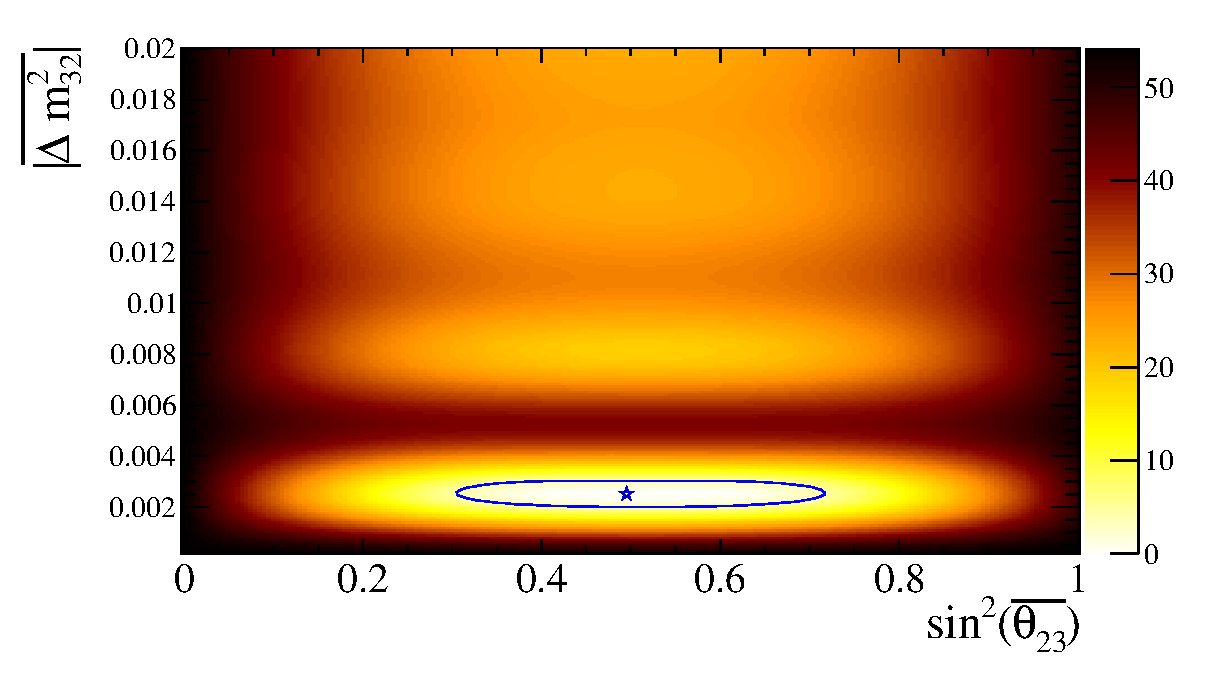
\includegraphics[width=36pc]{./images/asimov_fit/realdata_vs_asimov_nh_asimonly.eps}
    \caption {
      $\Delta\chi^2$ surface from the fit of the \TotalPot Asimov dataset.
      The normal mass hierarchy is assumed, with the oscillation parameters
      from the T2K run 1-4 joint fit with reactor constraint, which
      can be seen in table~\ref{tab:osc_params_fixed_values_reactor}.
    }
    \label{fig:results_asmiov_chisq:normal}
  \end{minipage}
  \vfill
  \begin{minipage}[t]{0.96\linewidth}
    \center
    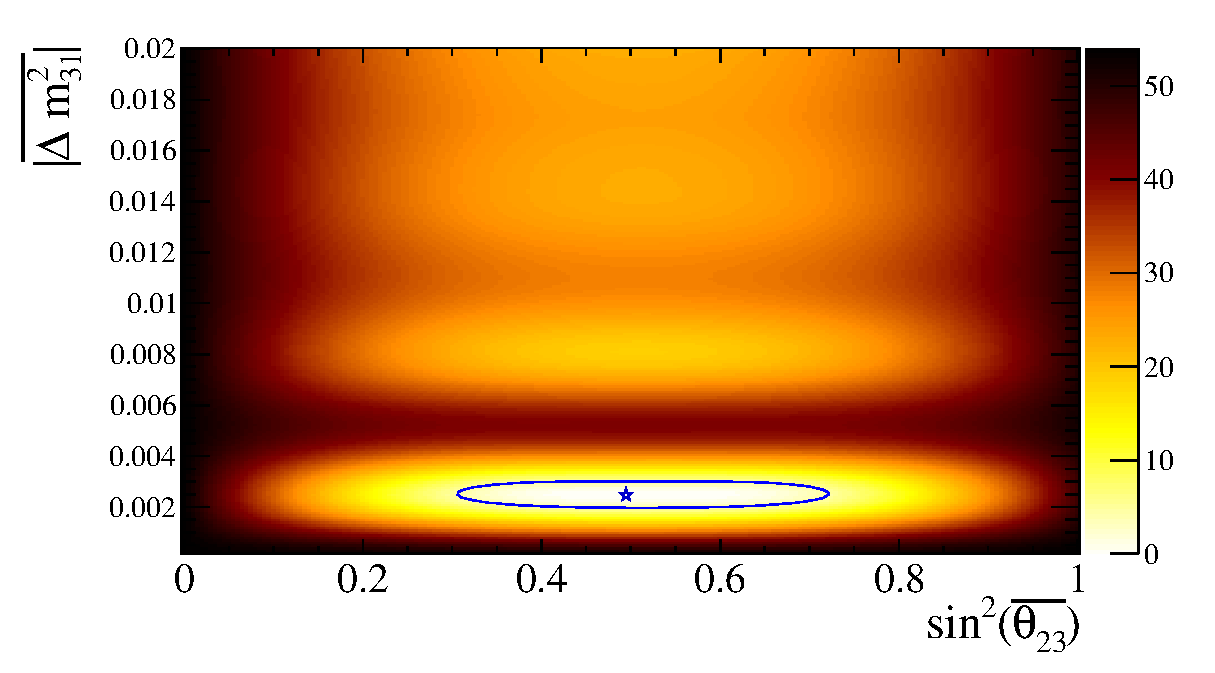
\includegraphics[width=36pc]{./images/asimov_fit/realdata_vs_asimov_ih_asimonly.eps}
    \caption {
      $\Delta\chi^2$ surface from the fit of the \TotalPot Asimov dataset.
      The inverted mass hierarchy is assumed, with the oscillation parameters
      from the T2K run 1-4 joint fit with reactor constraint, which
      can be seen in table~\ref{tab:osc_params_fixed_values_reactor}.
    }
    \label{fig:results_asmiov_chisq:inverted}
  \end{minipage}
\end{figure*}

%...........................................................
%
% Const-dchi^2 contours 
%

\clearpage

\begin{figure*}[htb]
\center
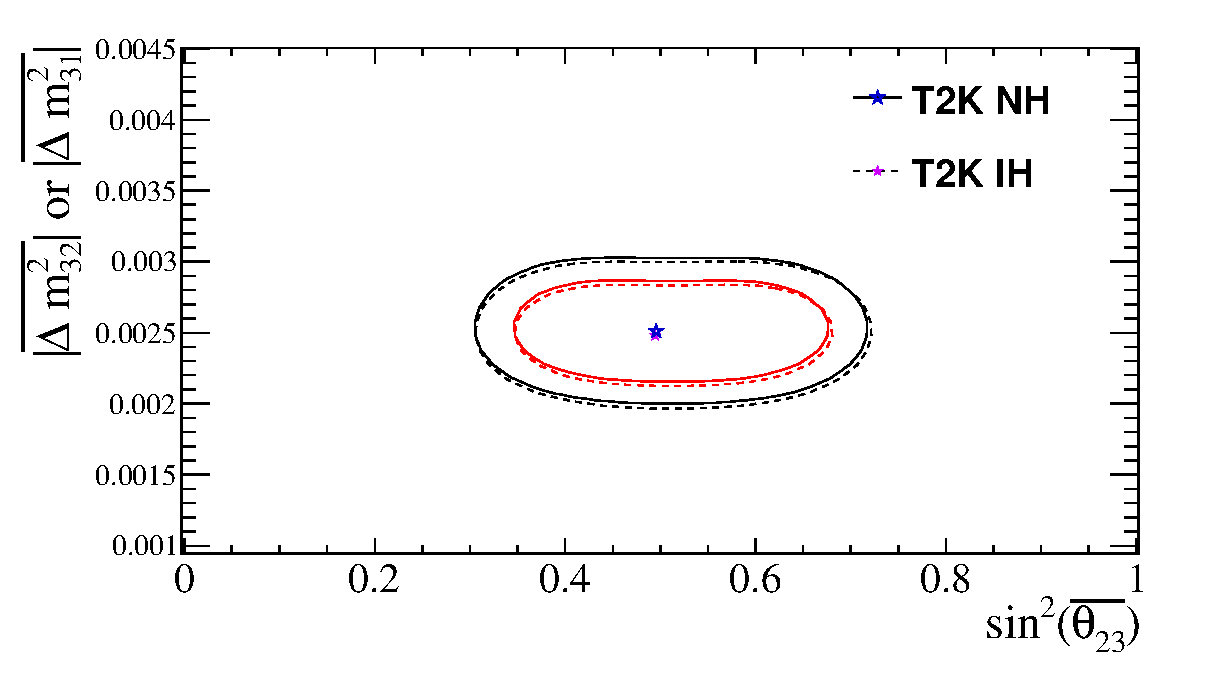
\includegraphics[height=0.35\textheight]{./images/asimov_fit/asimov_with_reactor_values.eps}
\caption {
  68\% CL and 90\% CL allowed regions, 
  constructed with the constant-$\Delta\chi^{2}$ method,
  from the fit of the \TotalPot Asimov dataset, 
  with the effects of statistical fluctuations and postfit systematic variations being included. 
  The best-fit point for each hypothesis is shown, with the larger point representing the better of the two fits.
}
\label{fig:results_asimov_contour}
\end{figure*}
\begin{figure*}[htb]
\center
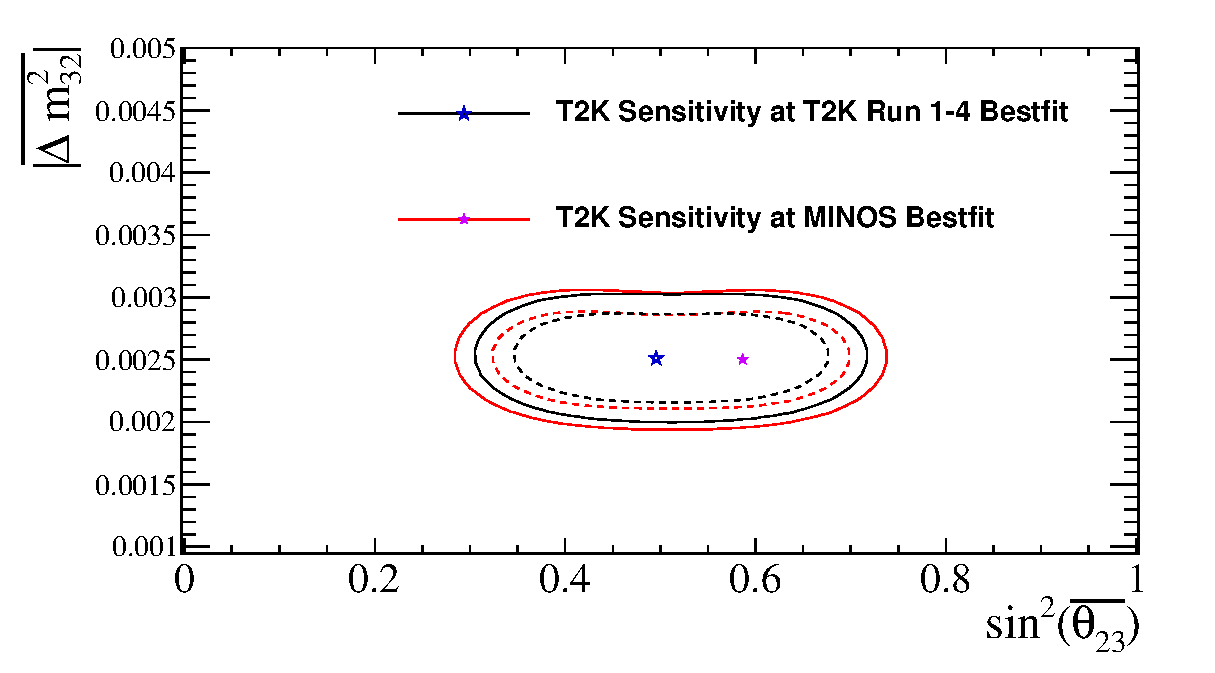
\includegraphics[height=0.35\textheight]{./images/asimov_fit/asimov_vs_asimov_at_minos_bf_zoomed_nh.eps}
\caption {
  68\% CL and 90\% CL allowed regions, 
  constructed with the constant-$\Delta\chi^{2}$ method,
  from the fit of the \TotalPot Asimov dataset, 
  with the effects of statistical fluctuations and postfit systematic variations being included.
  Contours are drawn with both the T2K run 1-4 oscillation parameters, and the MINOS antineutrino mode
  best-fit parameters ($\sin^2\theta_{23} = 0.587$, $\Delta m^2_{23} = 2.5 \times 10^{-3} \mathrm{eV^2}$).
  The normal hierarchy is assumed.
}
\label{fig:results_asimov_plusminos_nh}
\end{figure*}

\clearpage
\begin{figure*}[htb]
\center
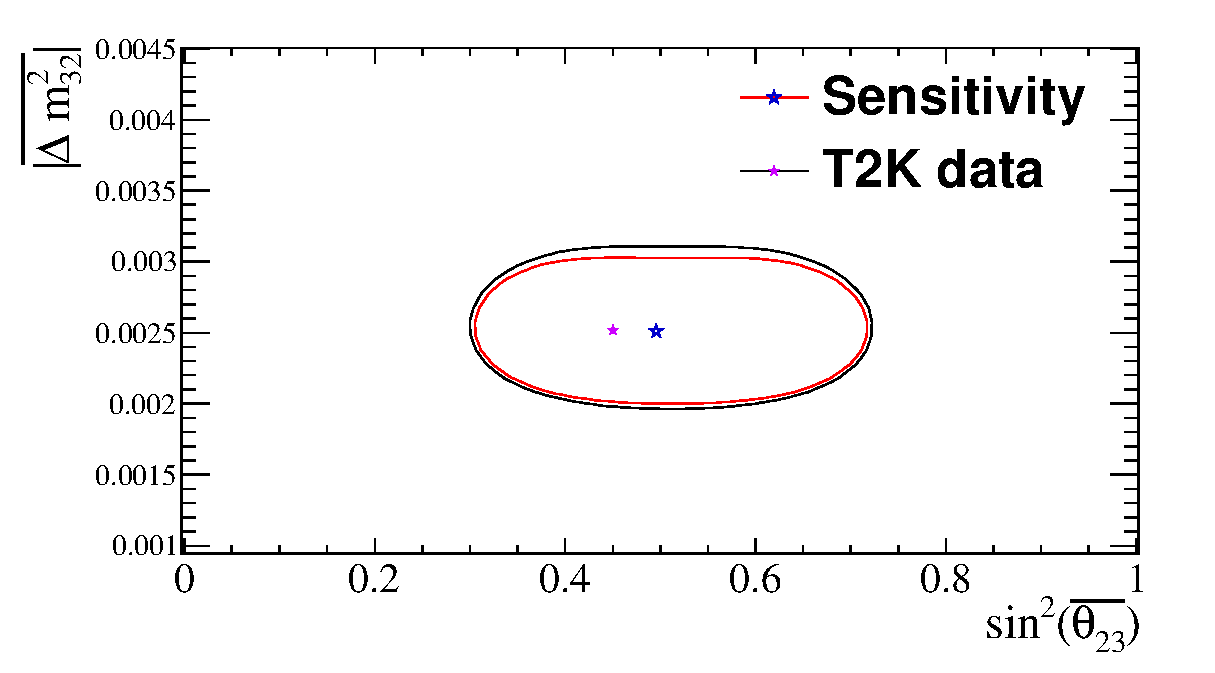
\includegraphics[height=0.34\textheight]{./images/asimov_fit/realdata_vs_asimov_zoomed_nh.eps}
\caption {
  68\% and 90\% CL allowed regions,
  constructed with the constant-$\Delta\chi^{2}$ method,
  from the fit to the Run 5+6 dataset, 
  with the effects of statistical fluctuations and postfit systematic variations being included. 
  These contours compare a fit to the Asimov dataset with the fit to the real data.
  The normal hierarchy is assumed.
  The oscillation parameters from the T2K run 1-4 joint fit with reactor constraint
  (table~\ref{tab:osc_params_fixed_values_reactor}) are used.
}
\label{fig:results_data_asimov_contour_nh}
\end{figure*}
\begin{figure*}[htb]
\center
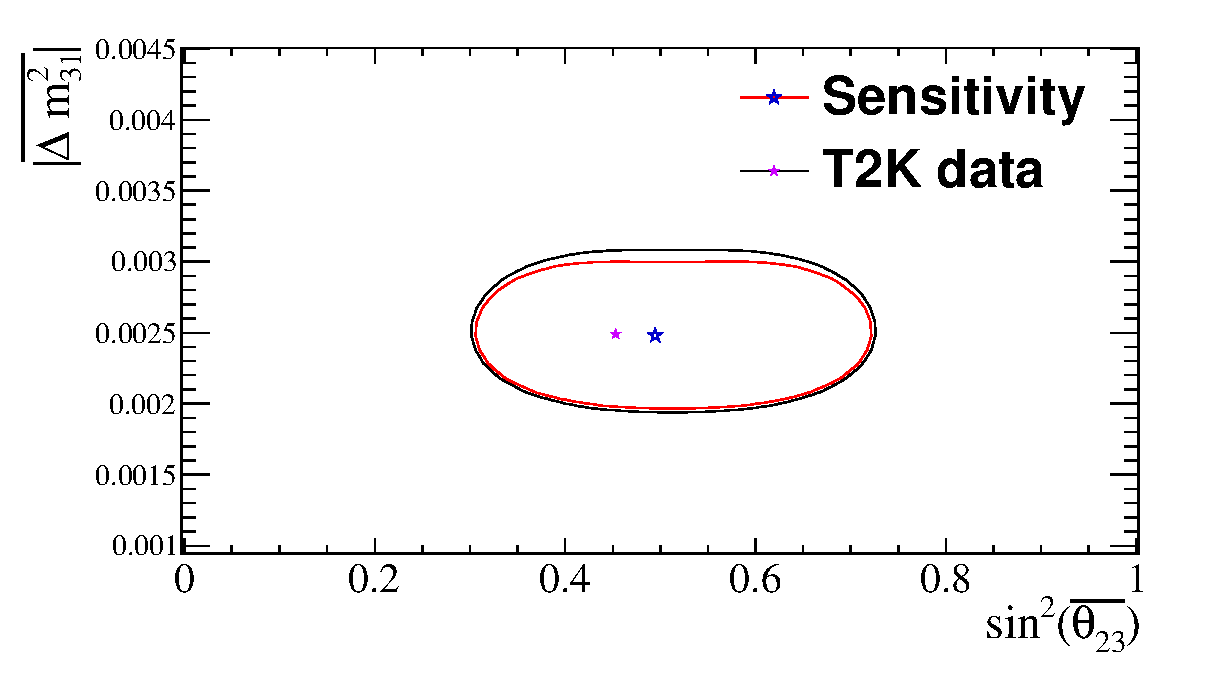
\includegraphics[height=0.34\textheight]{./images/asimov_fit/realdata_vs_asimov_zoomed_ih.eps}
\caption {
  68\% and 90\% CL allowed regions,
  constructed with the constant-$\Delta\chi^{2}$ method,
  from the fit to Run 5+6 dataset, 
  with the effects of statistical fluctuations and postfit systematic variations being included. 
  These contours compare a fit to the Asimov dataset with the fit to the real data.
  The inverted hierarchy is assumed.
  The oscillation parameters from the T2K run 1-4 joint fit with reactor constraint
  (table~\ref{tab:osc_params_fixed_values_reactor}) are used.
}
\label{fig:results_data_asimov_contour_ih}
\end{figure*}

\clearpage

% Asimov dataset fits with changing POT
%~ \begin{figure*}[htb]
%~ \center
%~ 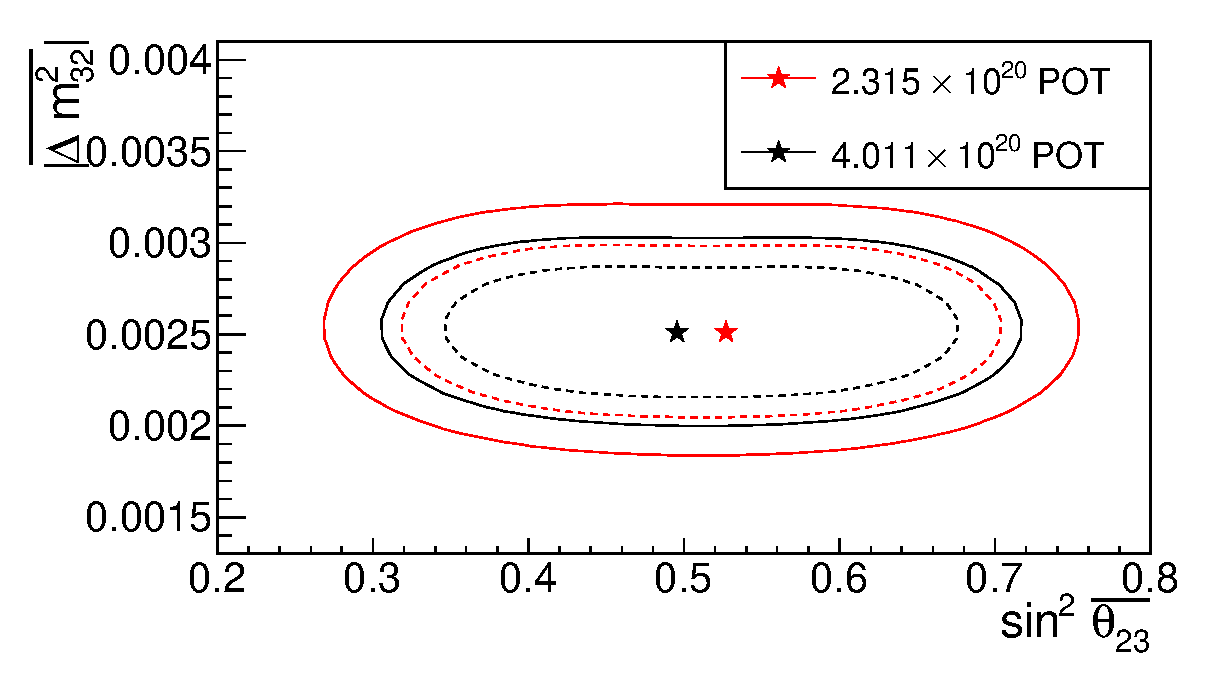
\includegraphics[height=0.36\textheight]{./images/asimov_fit/asimov_comparison_of_different_POT_nh.eps}
%~ \caption {
  %~ Comparison of the 68\% and 90\% Asimov dataset confidence regions with the data up to March 12, and the full Run 6 POT.
  %~ The normal mass hierarchy is assumed and
  %~ the oscillation parameters from the T2K run 1-4 joint fit with reactor constraint
  %~ (table~\ref{tab:osc_params_fixed_values_reactor}) are used.
%~ }
%~ \label{fig:results_asimov_changing_pot_nh}
%~ \end{figure*}
%~ 
%~ \begin{figure*}[htb]
%~ \center
%~ 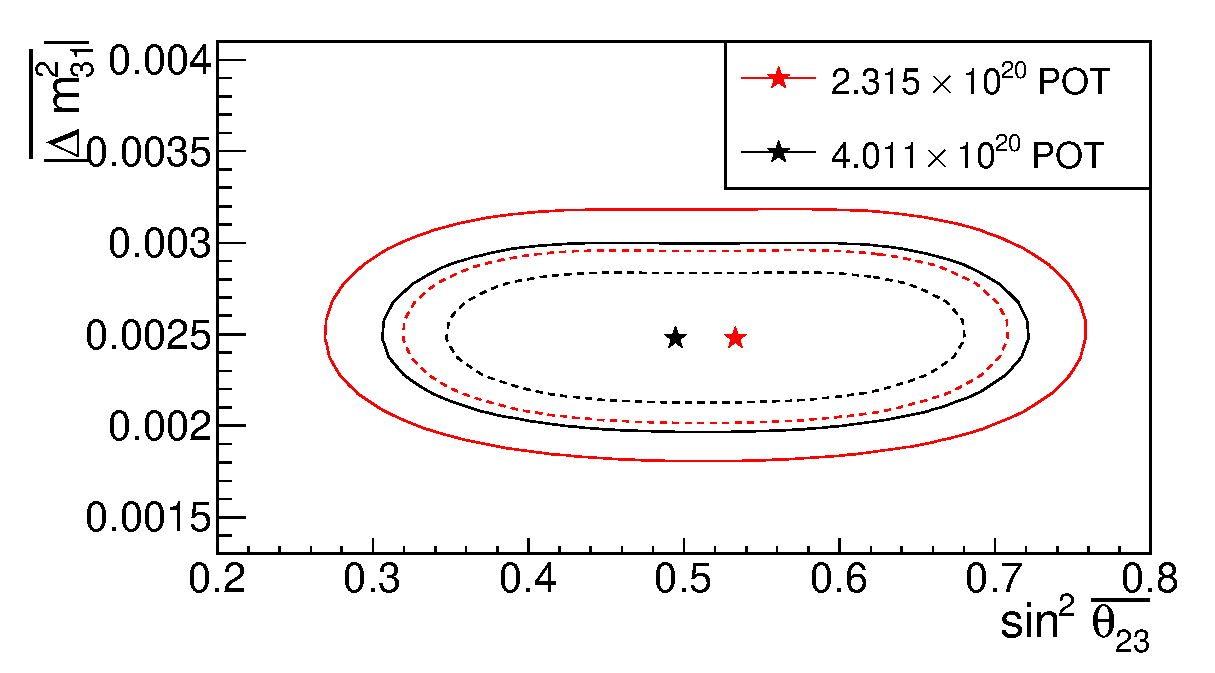
\includegraphics[height=0.36\textheight]{./images/asimov_fit/asimov_comparison_of_different_POT_ih.eps}
%~ \caption {
  %~ Comparison of the 68\% and 90\% Asimov dataset confidence regions with the data up to March 12, and the full Run 6 POT.
  %~ The inverted mass hierarchy is assumed and
  %~ the oscillation parameters from the T2K run 1-4 joint fit with reactor constraint
  %~ (table~\ref{tab:osc_params_fixed_values_reactor}) are used.
%~ }
%~ \label{fig:results_asimov_changing_pot_ih}
%~ \end{figure*}
